\documentclass[tikz,border=2pt]{standalone}
\usepackage{amsmath,amssymb}
\usepackage{tikz}
\usetikzlibrary{arrows.meta}

\begin{document}
% The kernel of the projection onto the x1-axis is the x2-axis: every vector on it is sent to 0.
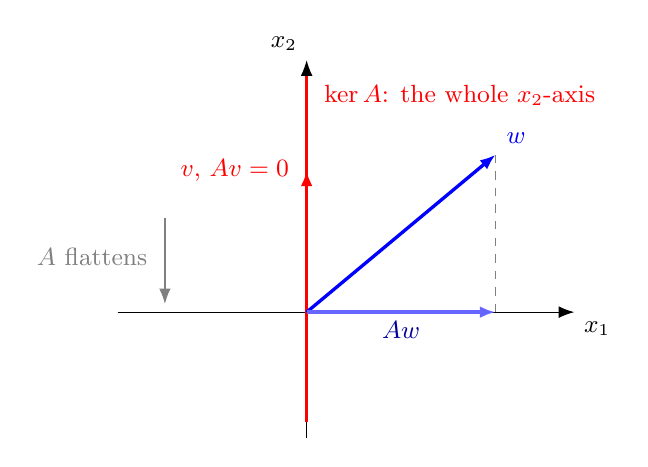
\begin{tikzpicture}[every node/.style={font=\small}, >={Latex[length=2mm]}]
	\draw[->] (-2.4,0) -- (3.4,0) node[below right] {$x_1$};
	\draw[->] (0,-1.6) -- (0,3.2) node[above left] {$x_2$};
	\draw[red, very thick] (0,-1.4) -- (0,3.0);
	\node[red, anchor=west] at (0.1,2.75) {$\ker A$: the whole $x_2$-axis};
	\draw[->, red, very thick] (0,0) -- (0,1.8);
	\node[red, anchor=east] at (-0.1,1.8) {$v$, $Av=0$};
	\draw[->, blue, very thick] (0,0) -- (2.4,2.0) node[above right] {$w$};
	\draw[->, blue!60, very thick] (0,0) -- (2.4,0);
	\node[blue!60!black, below] at (1.2,0) {$Aw$};
	\draw[dashed, gray] (2.4,2.0) -- (2.4,0);
	\draw[->, gray, thick] (-1.8,1.2) -- (-1.8,0.1);
	\node[gray, font=\small, anchor=east] at (-1.9,0.7) {$A$ flattens};
\end{tikzpicture}
\end{document}
